\chapter{Potenssiyhtälöt}

Ensimmäisen asteen yhtälöä $ax+b = 0$ monimutkaisempia yhtälöitä saadaan,
kun tuntematon $x$ korotetaan potenssiin.

\laatikko{\emph{Potenssiyhtälö} on muotoa 
$
x^n=a
$,
oleva yhtälö, jossa $n$ on positiivinen kokonaisluku. Eksponentin $n$ arvoa kutsutaan potenssiyhtälön \emph{asteeksi}.}

Potenssiyhtälöitä tarvitaan esimerkiksi tilanteissa, joissa lasketaan
korolle korkoa. Myös pinta-ala- ja tilavuuslaskuissa esiintyy potenssiyhtälöitä.

\begin{esimerkki}
\begin{enumerate}
\item[(a)]
Yhtälö $27x^3=7$ on potenssiyhtälö, sillä jakamalla se
puolittain luvulla $27$ saadaan $x^3 = \frac{7}{27}$.
\item[(b)]
Yhtälö $2x^{4}-7=3$ on potenssiyhtälö, sillä se voidaan muokata
muotoon $x^n = a$,
\begin{eqnarray*}
2x^{4} -7 &=& 3 \\
2x^{4} &=& 3+7 \\
x^{4} &=& \frac{10}{2} \\
x^{4} &=& 5.
\end{eqnarray*}
\item[(c)]
Yhtälö $x^{\frac{3}{2}}=42$ ei ole potenssiyhtälö, sillä eksponentti
$\frac{3}{2}$ ei ole kokonaisluku. Yhtälö voidaan kuitenkin kirjoittaa
uuden tuntemattoman $z=x^{\frac{1}{2}}=\sqrt{x}$ avulla: tällöin
saadaan potenssiyhtälö $z^3 = 42$.)
\item[(d)]
Yhtälö $x^{-2}=44$ ei ole potenssiyhtälö, sillä $-2$ ei ole positiivinen kokonaisluku. Sekin voidaan kirjoittaa potenssiyhtälönä, kun merkitään
$z=x^{-1}=\frac{1}{x}$. Tällöin saadaan yhtälö $z^2 = 44$.)
\end{enumerate}
\end{esimerkki}

\laatikko{\emph{Potenssiyhtälön ratkaiseminen}:
\begin{itemize}
\item
Jos potenssiyhtälön aste $n$ on \emph{parillinen} ja $a \ge 0$, yhtälöllä
on kaksi ratkaisua,
$$
x = \pm a^{\frac{1}{n}}\textrm{.}
$$ ($\pm$ tarkoittaa, että sekä positiivinen että negatiivinen 
arvo käyvät: $\pm 5$ tarkoittaa sekä lukuja $5$ että $-5$.)
\item
Jos aste on \emph{pariton}, yhtälöllä on täsmälleen yksi ratkaisu,
$$
x = a^{\frac{1}{n}}.
$$
\item
Jos aste on \emph{parillinen} ja $a < 0$, potenssiyhtälöllä ei ole yhtään
ratkaisua.
\end{itemize}}

\begin{esimerkki}
\begin{enumerate}
\item[(a)]
Potenssiyhtälön $x^3 = 100$ ratkaisu on $x=100^{\frac{1}{3}}=4{,}6416...$.
\item[(b)]
Potenssiyhtälöllä $x^4=50$ on kaksi ratkaisua $x=50^{\frac{1}{4}}=2{,}6591...$ ja $x=-50^{\frac{1}{4}}=-2{,}6591...$.
\item[(c)] 
Potenssiyhtälöllä $x^6 = -1$ ei ole ratkaisua, sillä $x^4 = (x^3)^2 \ge 0$ kaikille $x$.
\end{enumerate}

\begin{center}
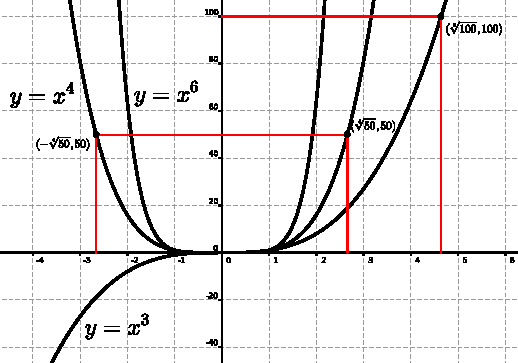
\includegraphics[width=12cm]{02-yhtalot/kuvia/xpot346.pdf}
\end{center}
\end{esimerkki}


\begin{esimerkki}
Suursijoittaja Nalle Mursulla on $5~000$ euroa ylimääräistä rahaa, jonka hän aikoo sijoittaa $30$ vuodeksi.  Nalle Mursu haluaa sijoittamansa pääoman kasvavan $100~000$ euroksi $30$ vuodessa.  Kuinka suuren vuotuisen korkokannan Nalle Mursu tarvitsee sijoitukselleen? 

\emph{Ratkaisu}:  Olkoon vuotuinen korkokanta $r$. \emph{Korkoa korolle -periaatteen} nojalla $5~000$ euron sijoitus kasvaa $30$ vuodessa summaksi $5~000\cdot(1+r)^{30}$.  Merkitsemällä $x=1+r$ saamme yhtälön $5~000\cdot x^{30} = 100~000$.  Jakamalla yhtälö puolittain luvulla $5~000$ päädymme 
potenssiyhtälöön 
$$
x^{30} = 20~000,
$$ 
jonka ratkaisuksi saadaan $x=20~000^{\frac{1}{30}} = 1{,}39\ldots$. Näin
ollen suursijoittaja Nalle Mursun vaatima korkokanta sijoitukselleen on noin $r=1-x=1-1,39=0,39=39~\%$.
\end{esimerkki}

%Potenssifunktiot ovat tapa katsoa potenssiyhtälöitä.

%\laatikko{\emph{Potenssifunktio} on funktio, jossa muuttuja $x$ korotetaan %potenssiin $n$. Potenssifunktion lauseke siis on
%$$
%f(x) = x^n.
%$$
%}

%Potenssiyhtälöä $x^n=a$ voidaan nyt tarkastella tarkastelemalla funktiota %$f(x)=x^n$ ja sen kuvaajaa $y=f(x)$. Tällöin siis $y=a$, eli $y$-akseli vastaa %$a$:n arvoja.

%\missingfigure{Funktioiden $f(x)={x}^3$ ja $g(x)=x^4$ kuvaajat.}

%\laatikko{
%\begin{itemize}
%\item
%Olkoon $n$ \emph{pariton}. Tällöin potenssifunktio $f(x)=x^n$ on kaikkialla %aidosti kasvava ja jatkuva. Tästä seuraa, että yhtälöllä $y=f(x)$ on aina tasan %yksi ratkaisu kaikilla $y$.    
%\item
%Olkoon $n$ \emph{parillinen}. Tällöin potenssifunktio $f(x)=x^n$ on positiivinen, %symmetrinen, jatkuva ja aidosti kasvava, kun $x$ on positiivinen.  %Positiivisuudesta seuraa, että yhtälöllä $y=f(x)$ ei ole ratkaisuja, jos $y$ on %negatiivinen. Symmetriasta $f(x)=f(-x)$ seuraa, että jos $x$ on ratkaisu, niin %myös $-x$ on ratkaisu.  
%\end{itemize}
%}

Yhtälöt, jotka ovat muotoa $a\cdot x^n = b$ (joskus myös muotoa ($a\cdot x^n - b = 0$), ratkaistavuus riippuu useammasta seikasta. Mikäli $n$ on pariton, yhtälö on aina ratkaistavissa (eli sillä on reaalinen juuri):
\begin{align*}
a\cdot x^n &= b \\
x^n &= \frac{b}{a} \\
x &= \sqrt[n]{\frac{b}{a}}
\end{align*}

\begin{esimerkki}
$2x^3 + 16 = 0 \Leftrightarrow 2x^3 = -16 \Leftrightarrow x^3 = -8  \Leftrightarrow x = \sqrt[3]{-8} = -2 $
\end{esimerkki}

Mikäli $n$ on parillinen, yhtälö on ratkaistavissa jos ja vain jos $\frac{b}{a} \geq 0 $. Parillisella potenssifunktiolla voi olla yksi, kaksi tai ei yhtään ratkaisua.

\begin{esimerkki}
$x^2 = 0 \Leftrightarrow x = 0 \\
\Rightarrow$ Yhtälöllä on yksi ratkaisu.
\end{esimerkki}

\begin{esimerkki}
$x^2 - 9 = 0 \Leftrightarrow x^2 = 9 \Leftrightarrow x = \pm 3 \\
\Rightarrow$ Yhtälöllä on kaksi ratkaisua, sillä $3^2 = 9$ ja $(-3)^2 = 9$.
\end{esimerkki}

\begin{esimerkki}
$x^2 + 9 = 0 \Leftrightarrow x^2 = -9 \Leftrightarrow x = \sqrt{-9} \\
\Rightarrow$ Yhtälöllä ei ole reaalista ratkaisua.
\end{esimerkki}

\section*{Tehtäviä}

\begin{tehtava}
Ratkaise: \\
a) $ x^2 = 4 $ \qquad
b) $ x^3 = 27 $ \qquad
c) $ x^5 = -1 $ \qquad
d) $ x^2 - 3 = 0 $ \qquad
e) $ x^3 + 125 = 0 $
\begin{vastaus}
a) $ x = 2 $ \qquad
b) $ x = 3 $ \qquad
c) $ x = -1 $ \qquad
d) $ x = \sqrt{3} $ \qquad
e) $ x = -5 $ 
\end{vastaus}
\end{tehtava}

\begin{tehtava}
Ratkaise \\
a) $ 5x^2 = 25 $ \qquad
b) $ (2x)^3 = 8 $ \qquad
c) $ x^4 = \frac{1}{4} $ \qquad
d) $ (3x)^2 = 36 $ \qquad
e) $ (4x)^2 + 16 = 0 $.
\begin{vastaus}
a) $ x = \sqrt{5} $ \qquad
b) $ x = 1 $ \qquad
c) $ x = \pm\frac{1}{\sqrt{2}} $ \qquad
d) $ x = 2 $ \qquad
e) Ei ratkaisua. 
\end{vastaus}
\end{tehtava}

\begin{tehtava}
Ratkaise potenssiyhtälöt
\begin{enumerate}
\item $x^3 = 81$
\item $x^5 = 10$
\item $x^2 = 4$
\item $x^4 = 1$.
\end{enumerate}
\end{tehtava}

\begin{tehtava}
Ratkaise potenssiyhtälöt
\begin{enumerate}
\item $x^4 - 8 = 0$
\item $2x^3 + 7 = 0$
\item $\frac{x^2}{4} - \frac{5}{2} = 1$
\item $1,51 x^4 - 1,2 = 7,5$.
\end{enumerate}
\end{tehtava}

\begin{tehtava}
Muinainen hallitsija Tauno Alpakka rakennuttaa itselleen kuution muotoista palatsia.  Palatsin tilavuuden tulee olla $5~000~\mathrm{m}^3$. 
\begin{enumerate}
\item Kuinka korkea palatsista tulee?
\item Palatsi päällystetään $10~\mathrm{cm}$:n paksuisella kultakerroksella.  Kuinka monta kiloa kultaa tarvitaan? (Kullan tiheys on $19,23 \cdot 10^3~\mathrm{ kg}/\mathrm{m}^3$.) 
\end{enumerate}
\end{tehtava}

